\mychapter{III. METHODOLOGY}{III. METHODOLOGY}

\section{Methodological Framework and System Architecture}
\hs This research designs, implements, and evaluates an automated, high-frequency price collection, econometric aggregation, and machine learning inflation forecasting system for Cambodia. The overarching methodology is organized around an end-to-end \textbf{Medallion Data Architecture}, structured into four progressive stages: multi-source automated data ingestion (Bronze Layer), data cleaning, unit normalization, and artificial intelligence classification (Silver Layer), axiomatic econometric index calculation and machine learning forecasting (Gold Layer), and interactive decision-support visualization (Serving Layer).

\begin{figure}[H]
    \centering
    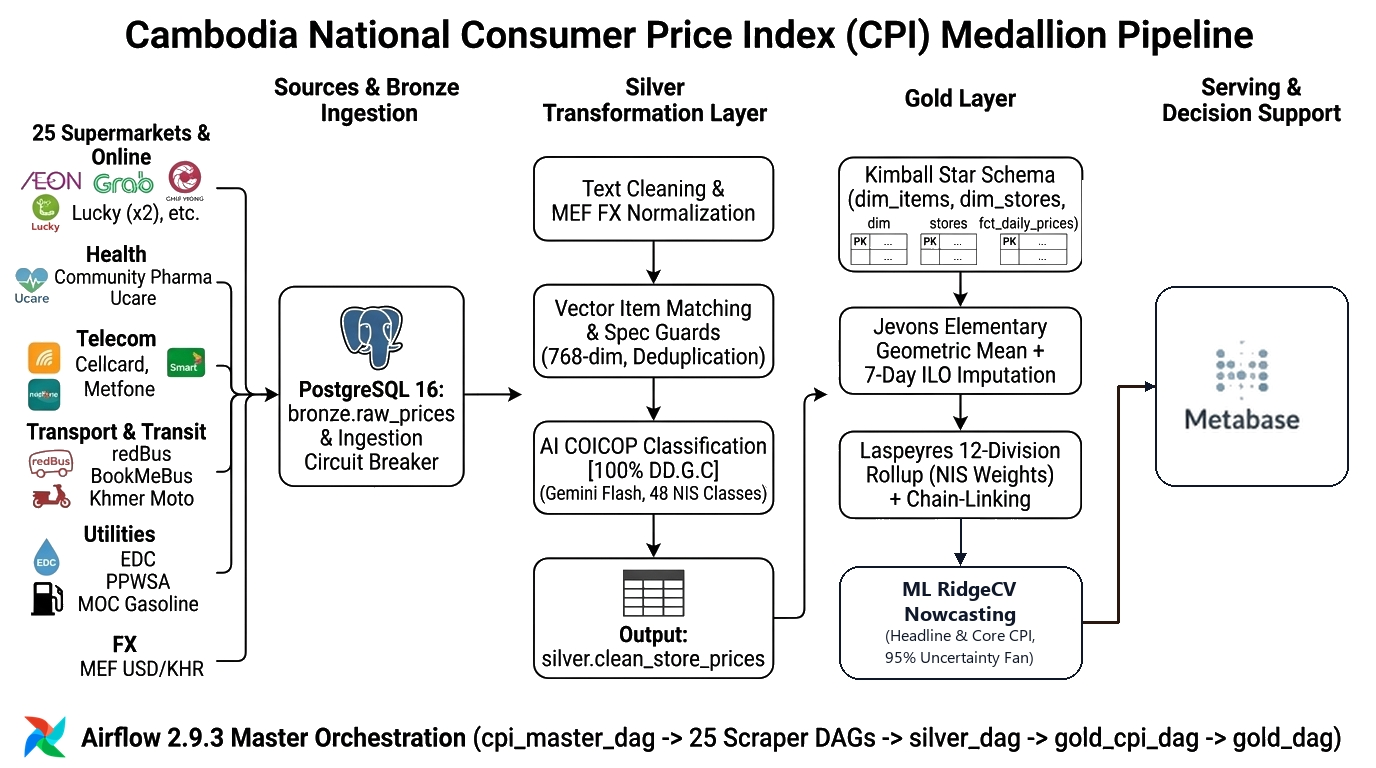
\includegraphics[width=\textwidth]{images/cpi_end_to_end_architecture_white.jpg}
    \caption{End-to-End Architecture and Dataflow of the Cambodia Daily CPI Medallion Pipeline.}
    \label{fig:cpi_architecture}
\end{figure}

\hs The architecture is designed to address the fundamental trade-off in economic measurement: combining the massive scale and daily speed of web-scraped big data with the strict mathematical rigor and international compliance required by national statistical institutions.

\section{Phase 1: Multi-Source Data Ingestion and Infrastructure Design}

\subsection{The Medallion Data Engineering Framework}
\hs In modern data science, managing large-scale, high-frequency web data requires a multi-stage data lakehouse architecture. The pipeline implements the three-tier Medallion architecture:
\begin{enumerate}
    \item \textbf{The Bronze Layer (Raw Storage):} Acts as the permanent, immutable landing zone for all incoming web extractions. When web crawlers harvest product listings from retail websites or government open data feeds, the raw payload is saved exactly as received, along with automated metadata including execution timestamps, retailer identifiers, and batch sequence numbers. No transformations, filters, or corrections are applied in this layer. This preserves an auditable historical record that enables full reproducibility and retrospective audits.
    \item \textbf{The Silver Layer (Cleaned and Validated Data):} Acts as the central data refinery. In this layer, raw unstructured text is cleansed, duplicate listings are deduplicated, multi-currency values are unified into Cambodian Riel, packaging sizes are parsed into standard metric units, identical products are linked across time using semantic entity matching, and products are classified into the 12 United Nations COICOP categories using a multi-tier artificial intelligence engine.
    \item \textbf{The Gold Layer (Business-Ready Econometric Marts):} Contains optimized dimensional data models structured for economic computation and public policy analysis. In this layer, elementary Jevons price relatives are compiled, missing price imputation algorithms are applied, national expenditure weights are integrated, Headline and Core CPI indices are calculated daily, and feature matrices are supplied to machine learning forecasting models.
\end{enumerate}

\subsection{Multi-Source Coverage: The 20 Market Sources}
\hs To ensure comprehensive coverage of Cambodian consumer spending, the ingestion engine collects price data daily across 20 distinct market sources spanning all 12 United Nations COICOP divisions:
\begin{itemize}
    \item \textbf{Modern Retail Supermarkets (Divisions 01, 02, 05, and 12):} AEON Online Store 1, AEON Store 3 Mean Chey, and DeliShop Asia. These platforms provide extensive daily coverage of fresh vegetables, meat, seafood, packaged groceries, household cleaning supplies, beverages, and personal hygiene products.
    \item \textbf{Digital E-Commerce Marketplaces (Divisions 03, 05, 09, and 12):} L192 Marketplace and Khmer24. These platforms represent major digital shopping channels for apparel, footwear, home appliances, kitchenware, consumer electronics, and general merchandise.
    \item \textbf{Healthcare and Pharmaceuticals (Division 06):} Community Pharmacy chain digital catalog. Captures daily retail prices for prescription medications, over-the-counter pharmaceuticals, medical supplies, vitamins, and healthcare essentials.
    \item \textbf{Inter-Provincial Transport and Transit (Division 07):} redBus Cambodia and BookMeBus digital ticketing platforms. Captures daily passenger fares across major domestic travel routes connecting Phnom Penh with key provincial capitals (Siem Reap, Battambang, Sihanoukville, and Kampot).
    \item \textbf{Housing Rentals and Real Estate (Division 04):} Khmer24 Real Estate and Realestate.com.kh. Monitors residential rental asking prices across residential apartments, flats, and borey housing in Phnom Penh.
    \item \textbf{Telecommunications and Digital Connectivity (Division 08):} Cellcard, Smart Axiata, and Metfone digital service portals, supplemented by retail smartphone listings from Ary Store and Khmer Samnang. Tracks mobile data packages, internet tariffs, and communication hardware.
    \item \textbf{Hospitality, Recreation, and Education (Divisions 09, 10, and 11):} Major hotel portals (Sokha Hotels, Hyatt Regency Phnom Penh), casual restaurant menus, and educational supply retailers.
    \item \textbf{Official Government Administrative Data Feeds (Divisions 07 and 12):} The Ministry of Commerce (MOC) bi-weekly regulated retail fuel price determinations (regular gasoline, premium gasoline, and diesel) and the Ministry of Economy and Finance (MEF) official daily foreign exchange rate (USD/KHR).
\end{itemize}

\subsection{Ingestion Resilience and Quality Control Mechanisms}
\hs Scraping external commercial websites involves technical risks, including website structure redesigns, intermittent network timeouts, and bot-detection challenges. To ensure uninterrupted daily operations, the pipeline incorporates several automated quality control guards:
\begin{itemize}
    \item \textbf{Circuit Breakers for Extraction Failures:} If an automated crawler returns zero products or an abnormally low quote count (for example, less than $50\%$ of historical volume), the system triggers a circuit breaker that halts downstream processing, logs an anomaly alert, and prevents corrupt or empty batches from overwriting historical price facts.
    \item \textbf{Automated Retry and Backoff Protocols:} Network requests implement exponential backoff retry algorithms to handle transient server errors, ensuring that temporary drops in retailer website availability do not cause permanent daily data gaps.
    \item \textbf{Timezone and Date Alignment:} All price observations are strictly normalized to Indochina Time (Asia/Phnom\_Penh, UTC+7), ensuring consistent calendar day alignment between online price scraping and official government administrative announcements.
\end{itemize}

\section{Phase 2: Data Preprocessing, Normalization, and AI Classification}

\subsection{Text Cleaning and Unit Standardization}
\hs Raw price listings harvested from the web are inherently noisy. The Silver layer applies a rigorous, multi-step data cleansing workflow:
\begin{enumerate}
    \item \textbf{Text Hygiene and Numeral Translation:} Cleans title strings by stripping marketing adjectives, promotional buzzwords (such as ``Best Seller'' or ``Mega Discount''), HTML escape sequences, and special characters. Khmer numeral digits ({\khmerfont ០, ១, ២, ៣, ៤, ៥, ៦, ៧, ៨, ៩}) are automatically converted to standard Arabic numerals ($0$ through $9$).
    \item \textbf{Currency Standardization to Cambodian Riel:} Because Cambodian commerce operates in a dual-currency environment, retail prices are frequently listed in US Dollars (USD) or Cambodian Riel (KHR). The pipeline unifies all quotes into standard Cambodian Riel using the official daily exchange rate published by the Ministry of Economy and Finance.
    \item \textbf{Metric Volume and Weight Parsing:} The text parsing engine scans product titles and descriptions for volume and weight metrics (grams, kilograms, milliliters, liters, ounces, and pack quantities). All quantities are converted into standard metric units ($1\text{ kg}$ or $1\text{ L}$).
    \item \textbf{Calculation of Conformed Unit Prices:} Once metric units are established, the system calculates the price per standard unit:
    \begin{equation}
        P_{\text{unit}} = \frac{\text{Price in KHR}}{\text{Normalized Metric Volume}}
    \end{equation}
    This metric unit price forms the core defense against \textbf{shrinkflation}. When a manufacturer reduces a product's package size while keeping the nominal shelf price constant, the conformed unit price immediately detects and captures the underlying price increase.
\end{enumerate}

\subsection{Semantic Entity Matching with Physical Specification Guards}
\hs To calculate true price changes over time, the system must track the exact same product from day to day. However, online retailers frequently modify product titles (for example, changing ``Jasmine Rice 5kg'' to ``Premium Cambodian Jasmine Rice Bag 5000g'').

\hs Standard text-matching algorithms often make catastrophic errors in retail data. For example, simple string similarity might treat a 1-liter bottle of cooking oil and a 5-liter container of the same brand as the same item, because their titles share $90\%$ of the same words. Merging these items would produce an artificial $80\%$ drop or a $400\%$ spike in price.

\hs To solve this problem, the pipeline develops a hybrid entity resolution engine combining:
\begin{itemize}
    \item \textbf{Dense Multilingual Vector Embeddings:} Product titles are converted into 768-dimensional dense mathematical vectors using advanced multilingual text embedding models. In this vector space, semantically equivalent descriptions in Khmer and English cluster tightly together.
    \item \textbf{Deterministic Specification Guards:} Before two listings can be merged as the same canonical product, they must pass strict physical attribute constraints:
    \begin{itemize}
        \item \textit{Metric Tolerance Guard:} The parsed volume or weight between the two items must match within a tight tolerance ($\le 10\%$). A 500ml bottle is never merged with a 1-liter bottle.
        \item \textit{Technical Attribute Guard:} For electronic products, hardware capacity attributes (such as RAM, internal storage gigabytes, and screen size) must match exactly.
        \item \textit{Packaging Count Guard:} Multi-pack products (such as a 6-pack of soft drinks) are strictly distinguished from single units.
    \end{itemize}
\end{itemize}
Only listings that satisfy both semantic vector similarity and all physical specification guards are linked into canonical product identities.

\subsection{The 4-Tier Hybrid AI COICOP Classification Engine}
\hs To classify thousands of diverse consumer goods into the 12 United Nations COICOP divisions, the pipeline deploys a 4-tier hierarchical classification ladder designed to maximize accuracy while minimizing computational delay and cost:
\begin{itemize}
    \item \textbf{Tier 1: Human Authority Override:} Verified classifications manually reviewed by economic analysts. This tier has highest priority and absolute confidence ($1.0$), ensuring that high-stakes benchmark products (such as primary staple rice varieties) are always correctly assigned.
    \item \textbf{Tier 2: Store Domain Purity Locking:} Specialized retail platforms operate within narrow, dedicated economic sectors. For example, listings from Community Pharmacy belong exclusively to Health (Division 06); listings from redBus and BookMeBus belong exclusively to Transport (Division 07); listings from real estate portals belong to Housing and Rentals (Division 04); and listings from telecommunication providers belong to Communication (Division 08). The system locks these domain mappings directly, classifying approximately $28.5\%$ of all incoming records with near-zero latency and $99.6\%$ precision without requiring artificial intelligence queries.
    \item \textbf{Tier 3: Multilingual Artificial Intelligence Inference with Database Memoization:} For generalized supermarket and marketplace catalogs (such as AEON and L192) that span multiple consumption divisions, the pipeline employs high-throughput Google Gemini artificial intelligence models. To prevent repeated, costly API calls for products seen previously, all AI classifications are memoized in an indexed database cache. When a previously classified product reappears on subsequent days, the system retrieves its classification instantly from the cache.
    \item \textbf{Tier 4: Retailer Category Fallback and Review Triage:} If an item is entirely new and cannot be classified with high confidence by Tier 3, the system falls back to the retailer's native website category mapping and places the record in a verification queue for analyst inspection.
\end{itemize}

\section{Phase 3: Econometric CPI Compilation and Missing Price Imputation}

\subsection{The Micro-Level: Elementary Jevons Index Calculation}
\hs Once clean price observations are assigned to their respective consumption categories, the Gold layer computes price relatives comparing current prices to the baseline period (August 18, 2026 = 100.00).

\hs At the elementary product level, the pipeline aggregates individual price quotes using the axiomatic unweighted geometric mean (\textbf{Jevons formula}):
\begin{equation}
    I_{s, t}^{\text{Jevons}} = \prod_{i \in s} \left( \frac{p_{i, t}}{p_{i, 0}} \right)^{\frac{1}{n_s}} = \frac{\left( \prod_{i \in s} p_{i, t} \right)^{\frac{1}{n_s}}}{\left( \prod_{i \in s} p_{i, 0} \right)^{\frac{1}{n_s}}} \times 100
\end{equation}
where $p_{i, t}$ is the price of product $i$ on day $t$, $p_{i, 0}$ is its base period price, and $n_s$ is the number of active price quotes in stratum $s$.

\hs As established in international index number theory, using the geometric mean rather than the arithmetic average (Carli index) guarantees that the elementary index satisfies the time-reversal and circularity axioms. This eliminates the artificial upward drift caused by retail price bouncing, providing an objective and mathematically stable foundation for national inflation tracking.

\subsection{Principled Missing Price Imputation Engine}
\hs In online retail environments, products frequently experience temporary stockouts, weekend inventory resets, or brief website maintenance. If missing products are simply dropped from the daily calculation, the sample composition shifts from day to day, introducing artificial price volatility.

\hs To preserve longitudinal time-series continuity, the pipeline implements a \textbf{7-day carry-forward imputation rule} recommended by the IMF CPI Manual \citep{imf2020cpi}:
\begin{itemize}
    \item If a product was observed on previous days but is temporarily unavailable on day $t$, its last observed price is carried forward for up to 7 consecutive calendar days.
    \item If the product returns to the catalog within the 7-day window, its real observed price resumes immediately.
    \item If the product remains absent for more than 7 consecutive days, it is flagged as permanently discontinued or out-of-season, and removed from the active daily calculation basket to prevent stale prices from accumulating.
\end{itemize}

\subsection{The Macro-Level: 12-Division Laspeyres Aggregation}
\hs At the upper level of aggregation, stratum indices are combined into the 12 United Nations COICOP division indices and the final National Headline CPI using the fixed-base \textbf{Modified Laspeyres} formula:
\begin{equation}
    \text{CPI}_t^{\text{Headline}} = \sum_{d=1}^{12} w_d \cdot I_{d, t}
\end{equation}
where $w_d$ represents the official household expenditure weight for COICOP division $d$ normalized to sum to exactly $1.00000$ ($100.000\%$). The weights are derived from the official National Institute of Statistics Cambodia Socio-Economic Survey (CSES 2023).

\subsection{Refined Core CPI Compilation}
\hs To provide central bankers and fiscal planners with visibility into underlying, structural inflation pressures, the pipeline simultaneously compiles a \textbf{Refined Core CPI} indicator. The Core CPI excludes volatile food categories and regulated energy components:
\begin{equation}
    \text{CPI}_t^{\text{Core}} = \frac{\sum_{d \notin \{\text{Food, Energy}\}} w_d \cdot I_{d, t}}{\sum_{d \notin \{\text{Food, Energy}\}} w_d}
\end{equation}
By excluding Division 01 (Food and Non-Alcoholic Beverages: $44.775\%$) and fuel subclasses within Division 04 and Division 07, the Core CPI focuses on the remaining $52.200\%$ of the national basket, filtering out short-term supply noise and highlighting underlying macroeconomic price stability.

\section{Phase 4: High-Frequency Inflation Forecasting via Machine Learning}

\subsection{Direct Multi-Horizon Forecasting Formulation}
\hs While traditional macroeconomic forecasting relies on low-frequency quarterly or monthly aggregates, high-frequency price intelligence demands real-time predictive models capable of projecting price trajectories over multi-day horizons \citep{medeiros2021forecasting, gouletcoulombe2022machine}. To deliver actionable foresight to central bankers and fiscal planners, the pipeline deploys an autonomous supervised machine learning forecasting engine directly driven by high-frequency daily price facts from \texttt{gold.fct\_cpi\_daily}.

\hs Rather than employing iterative recursive autoregressions---which suffer from rapid error compounding across extended horizons---the system implements a \textbf{Direct Multi-Horizon Forecasting Strategy}. For each reference calculation date $t$ and forecast horizon $H \in \{7, 14, 30\}$ days, the supervised target variable $y_t^{(H)}$ is defined as the forward cumulative percentage change in the National Headline CPI:
\begin{equation}
    y_t^{(H)} = \left( \frac{\text{CPI}_{t+H} - \text{CPI}_t}{\text{CPI}_t} \right) \times 100\%
\end{equation}
Given the estimated forward inflation rate $\hat{y}_t^{(H)}$, the projected CPI index level at horizon $H$ is computed directly as:
\begin{equation}
    \widehat{\text{CPI}}_{t+H} = \text{CPI}_t \times \left( 1 + \frac{\hat{y}_t^{(H)}}{100} \right)
\end{equation}
This formulation ensures that forecasts are tied directly to realized index levels, providing both relative rate and absolute index projections for 7-day (weekly), 14-day (bi-weekly), and 30-day (monthly) policy planning windows.

\subsection{High-Frequency Feature Engineering and Econometric Signals}
\hs The predictive power of machine learning models in macroeconomic environments depends fundamentally on feature representation \citep{babii2022machine}. The pipeline extracts a rich multidimensional feature vector $\mathbf{x}_t \in \mathbb{R}^D$ from the daily price history, strictly shifted by one observation ($t-1$) to guarantee zero look-ahead bias:

\begin{enumerate}
    \item \textbf{Base Daily Returns and Autoregressive Lags:} The immediate day-over-day price return is computed as:
    \begin{equation}
        r_t = \left( \frac{\text{CPI}_t - \text{CPI}_{t-1}}{\text{CPI}_{t-1}} \right) \times 100\%
    \end{equation}
    To capture short-term price memory and momentum persistence, autoregressive lag features are constructed across expanding intervals:
    \begin{equation}
        L_k(t) = r_{t-k}, \quad \text{for } k \in \{1, 2, 3, 7, 14, 30\}
    \end{equation}

    \item \textbf{Multi-Horizon Moving Averages and Trend Velocity:} To filter high-frequency noise from structural trends, trailing simple moving averages are computed over 7-day, 14-day, and 30-day windows:
    \begin{equation}
        \text{MA}_k(t) = \frac{1}{k} \sum_{i=1}^{k} \text{CPI}_{t-i}, \quad k \in \{7, 14, 30\}
    \end{equation}
    The relative velocity between short-term and medium-term price trends is captured by the normalized momentum spread:
    \begin{equation}
        \text{Spread}_{7,30}(t) = \left( \frac{\text{MA}_7(t) - \text{MA}_{30}(t)}{\text{MA}_{30}(t)} \right) \times 100\%
    \end{equation}

    \item \textbf{Rolling Volatility Estimators:} High-frequency market turbulence and price dispersion are measured by the rolling sample standard deviation of daily returns:
    \begin{equation}
        \sigma_k(t) = \sqrt{\frac{1}{k-1} \sum_{i=1}^{k} \left( r_{t-i} - \bar{r}_k(t) \right)^2}, \quad k \in \{7, 14\}
    \end{equation}

    \item \textbf{Cross-Division Leading Momentum Signals:} In developing economies, aggregate inflation is predominantly led by supply-side shocks in food and energy \citep{cavallo2016billion, macias2023nowcasting}. The pipeline computes dedicated 7-day cumulative momentum signals for Division 01 (Food and Non-Alcoholic Beverages, $44.775\%$ basket weight) and Division 07 (Transport, $12.180\%$ basket weight):
    \begin{equation}
        M_{\text{Food}, t}^{(7)} = \left( \frac{I_{\text{Food}, t-1} - I_{\text{Food}, t-8}}{I_{\text{Food}, t-8}} \right) \times 100\%
    \end{equation}
    \begin{equation}
        M_{\text{Trans}, t}^{(7)} = \left( \frac{I_{\text{Trans}, t-1} - I_{\text{Trans}, t-8}}{I_{\text{Trans}, t-8}} \right) \times 100\%
    \end{equation}
    These two divisions account for nearly $57\%$ of the entire consumer basket, allowing their localized dynamics to serve as high-conviction leading indicators for headline movements.

    \item \textbf{Calendar Dynamics and Cambodian Cultural Festivals:} Seasonal consumer demand shifts are modeled using calendar indicators (day-of-week, weekend dummy, day-of-month) and smooth cyclical trigonometric encodings:
    \begin{equation}
        \sin_m(t) = \sin\left( \frac{2\pi \cdot m_t}{12} \right), \quad \cos_m(t) = \cos\left( \frac{2\pi \cdot m_t}{12} \right)
    \end{equation}
    where $m_t \in \{1, \dots, 12\}$ is the calendar month. Furthermore, binary indicators $\mathbb{I}_{\text{Festival}}(t)$ flag active expenditure windows surrounding major Cambodian holidays (Khmer New Year in mid-April, Pchum Ben in September/October, and the Water Festival in November), capturing documented seasonal retail demand surges.
\end{enumerate}

\subsection{Non-Linear Gradient Boosted Decision Trees (LightGBM Architecture)}
\hs Empirical macroeconomic research demonstrates that tree-based ensemble algorithms systematically outperform traditional linear and deep learning models on tabular economic time series with sharp regime shifts \citep{medeiros2021forecasting, gouletcoulombe2022machine}. The pipeline implements \textbf{LightGBM} (Light Gradient Boosting Machine), which optimizes an ensemble of $M$ decision trees:
\begin{equation}
    \hat{y}_t^{(H)} = \sum_{m=1}^{M} f_m(\mathbf{x}_t), \quad f_m \in \mathcal{F}
\end{equation}
At each boosting iteration $m$, the model minimizes a second-order Taylor approximation of the Mean Squared Error (MSE) objective with $L_2$ tree regularization:
\begin{equation}
    \mathcal{L}^{(m)} \approx \sum_{i=1}^{N} \left[ g_i f_m(\mathbf{x}_i) + \frac{1}{2} h_i f_m^2(\mathbf{x}_i) \right] + \gamma T + \frac{1}{2} \lambda \sum_{j=1}^{T} w_j^2
\end{equation}
where $g_i$ and $h_i$ represent the first and second-order loss gradients, $T$ denotes the number of terminal leaves, $w_j$ are the leaf weights, and $\lambda = 1.0$ penalizes model complexity. LightGBM utilizes Gradient-based One-Side Sampling (GOSS) and Exclusive Feature Bundling (EFB), ensuring sub-second model training and low latency during daily production runs. Hyperparameters are tuned with learning rate $\eta = 0.05$, max leaves $J = 31$, and minimum child samples $= 5$ to mitigate overfitting on limited time-series horizons.

\subsection{Walk-Forward Cross-Validation and Out-of-Sample Evaluation}
\hs A critical hazard in financial and economic forecasting is data leakage: standard randomized $K$-fold cross-validation uses future observations to predict the past, producing severely over-optimistic accuracy metrics. To ensure empirical validity, the pipeline enforces strict \textbf{Walk-Forward Time-Series Cross-Validation} via \texttt{TimeSeriesSplit} \citep{babii2022machine}.

\hs The historical sample is partitioned into $K$ sequential expanding temporal folds. In each fold $k$, the model trains exclusively on historical facts up to date $t_k$ and evaluates out-of-sample predictions on the subsequent window $[t_k + 1, t_k + H]$. Out-of-sample performance is tracked using Root Mean Squared Error (RMSE) and Mean Absolute Error (MAE):
\begin{equation}
    \text{RMSE}^{(H)} = \sqrt{\frac{1}{N_H} \sum_{i=1}^{N_H} \left( y_i^{(H)} - \hat{y}_i^{(H)} \right)^2}
\end{equation}
\begin{equation}
    \text{MAE}^{(H)} = \frac{1}{N_H} \sum_{i=1}^{N_H} \left| y_i^{(H)} - \hat{y}_i^{(H)} \right|
\end{equation}
This rigorous backtesting framework guarantees that all reported metrics reflect genuine out-of-sample predictive capability.

\subsection{Automated Production Serving and Database Persistence}
\hs Following feature generation, walk-forward validation, and full-sample re-fitting, the resulting multi-horizon predictions are upserted into the PostgreSQL Gold analytical mart:
\begin{equation}
    \texttt{gold.fct\_cpi\_forecast} \left( \text{execution\_date}, \text{target\_date}, H, \text{current\_cpi}, \hat{y}^{(H)}, \widehat{\text{cpi}}^{(H)}, \text{rmse}, \text{mae} \right)
\end{equation}
The forecasts are exposed via the analytical view \texttt{gold.v\_cpi\_forecast\_chart}, connecting historical daily CPI observations with forward 7-day, 14-day, and 30-day projection curves for direct consumption by BI dashboards and policy analysts.

\subsection{High-Frequency Inflation Nowcasting and Benchmark Chain-Linking}
\hs While multi-horizon machine learning models project forward price paths, fiscal authorities and the central bank require zero-lag estimates of the official monthly inflation rate before statistical agencies publish delayed reports \citep{cavallo2016billion, macias2023nowcasting}. To solve this 30-to-60-day reporting delay, the pipeline incorporates an intra-month \textbf{High-Frequency Inflation Nowcasting Engine} (\texttt{ml/nowcaster.py}).

\hs For an active calendar month $M$ with $T$ total days, on any calculation day $t \le T$, the full-month nowcast $\widehat{\text{CPI}}_M(t)$ is computed by partitioning the month into observed and unobserved days:
\begin{equation}
    \widehat{\text{CPI}}_M(t) = \left( \frac{t}{T} \right) \overline{\text{CPI}}_{\text{realized}}(t) + \left( \frac{T - t}{T} \right) \widehat{\text{CPI}}_{\text{remaining}}
\end{equation}
where $\overline{\text{CPI}}_{\text{realized}}(t) = \frac{1}{t} \sum_{\tau=1}^t \text{CPI}_\tau$ represents the mean of daily facts accumulated so far, and $\widehat{\text{CPI}}_{\text{remaining}}$ is projected using the high-frequency momentum of Food (Division 01) and Transport (Division 07). 

\hs The estimated Month-over-Month (MoM \%) nowcast is then derived relative to the prior month's monthly CPI:
\begin{equation}
    \widehat{\pi}_{\text{MoM}, M}(t) = \left( \frac{\widehat{\text{CPI}}_M(t) - \text{CPI}_{M-1}}{\text{CPI}_{M-1}} \right) \times 100\%
\end{equation}
To make the output directly comparable to official government releases, the nowcast is chain-linked to the historical National Institute of Statistics (NIS) Phnom Penh benchmark (Base Oct--Dec 2006 = 100):
\begin{equation}
    \widehat{\text{CPI}}_{\text{NIS}, M}(t) = \text{CPI}_{\text{NIS}, M-1} \times \left( 1 + \frac{\widehat{\pi}_{\text{MoM}, M}(t)}{100} \right)
\end{equation}
Dynamic 95\% confidence intervals are calculated using daily return volatility $\sigma_{\text{daily}}$ and the uncertainty decay ratio $U_t = \sqrt{(T - t)/T}$:
\begin{equation}
    \text{CI}_{95\%} = \widehat{\text{CPI}}_M(t) \pm 1.96 \cdot \sigma_{\text{daily}} \sqrt{\frac{T - t}{T}}
\end{equation}
All computed nowcasts are automatically persisted into \texttt{gold.fct\_cpi\_nowcast} and audited against official NIS publications in \texttt{gold.v\_nowcast\_evaluation}.

\section{Phase 5: Interactive Dashboard Architecture and Production Deployment}

\subsection{Executive Business Intelligence Dashboards}
\hs To ensure that the analytical outputs of the pipeline are immediately usable by economic policymakers, the system deploys interactive visualization dashboards in Metabase and Power BI:
\begin{itemize}
    \item \textbf{Executive Macro Overview:} Real-time dial gauges displaying current Headline and Core inflation rates, day-on-day changes, 30-day cumulative trends, and foreign exchange movements.
    \item \textbf{12-Division Drill-Down Analytics:} Interactive time-series charts allowing analysts to click into any specific COICOP division, view historical trajectories, and identify top rising or falling goods.
    \item \textbf{Operational Scraper Observability Matrix:} Displays the daily status of all 20 scrapers, recording daily quote yields, HTTP response codes, scraping execution duration, and data quality check results.
\end{itemize}

\subsection{Containerized Infrastructure}
\hs The complete ecosystem is containerized using Docker Compose, integrating PostgreSQL 16 (Medallion database storage), Apache Airflow 2.9.3 (workflow scheduling and DAG execution), automated transformation engines, and Metabase (business intelligence serving). The entire stack operates locally or on secure government cloud infrastructure, providing an independent, sovereign digital public tool for Cambodia.

\section{Methodological Activity Schedule}
\hs Table~\ref{table:methodology_roadmap} details the project execution timeline across the 12-week operational schedule.

\begin{table}[H]
\centering
\small
\begin{tabular}{|p{4.2cm}|*{10}{>{\centering\arraybackslash}p{0.75cm}|}}
\hline
\rowcolor{blue!20}
\textbf{Activity / Milestone} & \textbf{W1--2} & \textbf{W3} & \textbf{W4} & \textbf{W5} & \textbf{W6} & \textbf{W7} & \textbf{W8} & \textbf{W9} & \textbf{W10} & \textbf{W11--12} \\
\hline
\textbf{Data Ingestion \& Scraping} & \progressbar{ } & \progressbar{ } & \progressbar{ } & & & & & & & \\
\hline
\textbf{Silver Cleaning \& AI} & & \progressbar{ } & \progressbar{ } & \progressbar{ } & & & & & & \\
\hline
\textbf{Gold Econometric Jevons} & & & & \progressbar{ } & \progressbar{ } & \progressbar{ } & & & & \\
\hline
\textbf{ML Forecast \& BI Serving} & & & & & & \progressbar{ } & \progressbar{ } & \progressbar{ } & & \\
\hline
\textbf{Evaluation \& Defense} & & & & & & & & \progressbar{ } & \progressbar{ } & \progressbar{ } \\
\hline
\end{tabular}
\caption{Methodology Execution Schedule and Deliverable Milestones}
\label{table:methodology_roadmap}
\end{table}
